\documentclass{beamer}

\usepackage[resetfonts]{cmap}
\usepackage{lmodern}
\usepackage[english]{babel}
\usepackage{amsmath}
\usepackage{amsfonts}
\usepackage{graphicx}

%\AtBeginDocument{\shorthandoff{-"}} % Obejití chyby v podpoře češtiny v balíčku Babel.

\usepackage[latin2]{inputenc}
\usepackage[T1]{fontenc}
\usepackage[protrusion,expansion,step=1]{microtype}
\usepackage{hyperref}
\hypersetup{
  unicode=true,
  plainpages=false,
  pdfpagelabels=true,
  pdfpagemode=UseNone,
  pdfstartview=Fit,
  pdfpagelayout=SinglePage,
  pdfdisplaydoctitle=true,
  linkcolor={1 0 0},
  bookmarks=true,
  bookmarksopen=true,
  bookmarksopenlevel=1,
  bookmarksnumbered=true,
  pdfsubject={Image and Signal Processing, Convolution, Impulse Responses},
  pdfkeywords={Convolution, Dirac function}
}

%\usetheme{default}
%\usetheme{AnnArbor}
%\usetheme{Antibes}
%\usetheme{Bergen}
%\usetheme{Berkeley}
\usetheme{Berlin}
%\usetheme{Boadilla}
%\usetheme{CambridgeUS}
%\usetheme{Copenhagen}
%\usetheme{Darmstadt}
%\usetheme{Dresden}
%\usetheme{Frankfurt}
%\usetheme{Goettingen}
%\usetheme{Hannover}
%\usetheme{Ilmenau}
%\usetheme{JuanLesPins}
%\usetheme{Luebeck}
%\usetheme{Madrid}
%\usetheme{Malmoe}
%\usetheme{Marburg}
%\usetheme{Montpellier}
%\usetheme{PaloAlto}
%\usetheme{Pittsburgh}
%\usetheme{Rochester}
%\usetheme{Singapore}
%\usetheme{Szeged}
%\usetheme{Warsaw}

\usefonttheme{default}
%\usefonttheme{professionalfonts}
%\usefonttheme{serif}
%\usefonttheme{structurebold}
%\usefonttheme{structureitalicserif}
%\usefonttheme{structuresmallcapsserif}

%\usecolortheme{default}
%\usecolortheme{albatross}
\usecolortheme{beaver}
%\usecolortheme{beetle}
%\usecolortheme{crane}
%\usecolortheme{dolphin}
%\usecolortheme{dove}
%\usecolortheme{fly}
%\usecolortheme{lily}
%\usecolortheme{orchid}
%\usecolortheme{rose}
%\usecolortheme{seagull}
%\usecolortheme{seahorse}
%\usecolortheme{sidebartab}
%\usecolortheme{structure}
%\usecolortheme{whale}
%\usecolortheme{wolverine}

%\useinnertheme{default}
\useinnertheme{circles}
%\useinnertheme{inmargin}
%\useinnertheme{rectangles}
%\useinnertheme{rounded}

\useoutertheme{default}
%\useoutertheme{infolines}
%\useoutertheme{miniframes}
%\useoutertheme{shadow}
%\useoutertheme{sidebar}
%\useoutertheme{smoothbars}
%\useoutertheme{smoothtree}
%\useoutertheme{split}
%\useoutertheme{tree}
%\useoutertheme[subsection=false]{miniframes}

\setbeamercovered{transparent}
\setbeamertemplate{navigation symbols}{} % Odstranění navigační lišty.
%\setbeamertemplate{frametitle continuation}[from second]

\newcommand{\cssplit}[1]{\discretionary{#1}{#1}{#1}\kern 0pt} % Definice makra pro sazbu znaků opakovaných při zlomu na začátku dalsího řádku.
\newcommand{\spj}{\cssplit{-}} % Definice makra pro sazbu pri zlomu opakovaného  spojovníku.
\def\makro#1{\texttt{\char`\\#1}} % Makro pro sazbu názvů maker.
\let\bibautor\textsc % Vyznačení autora v seznamu literatury.
\let\bibnazev\textit % Vyznačení názvu díla v seznamu literatury.

\author{J\'an Bella \and Maxime Portaz}
\title{Delaunay Triangulation of Imprecise Points}
\subtitle{Preprocess and actually get a fast query time}
\institute{Grenoble INP}
\date{January 23, 2015} 

\setbeamerfont{footnote}{size=\tiny}

\makeatletter
\beamer@theme@subsectionfalse
\makeatother
		
\begin{document}
\frame{\titlepage}
\begin{frame}{Problem}
\begin{columns}
\column{.5\textwidth}
Given: 
a set of regions (imprecise points)\\
\pause
~\\
Is there an advantage we can take and find Delaunay triangulation effectively?
\column{.5\textwidth}
\begin{figure}
		\centering
\hspace*{-0.5cm}		\only<1>{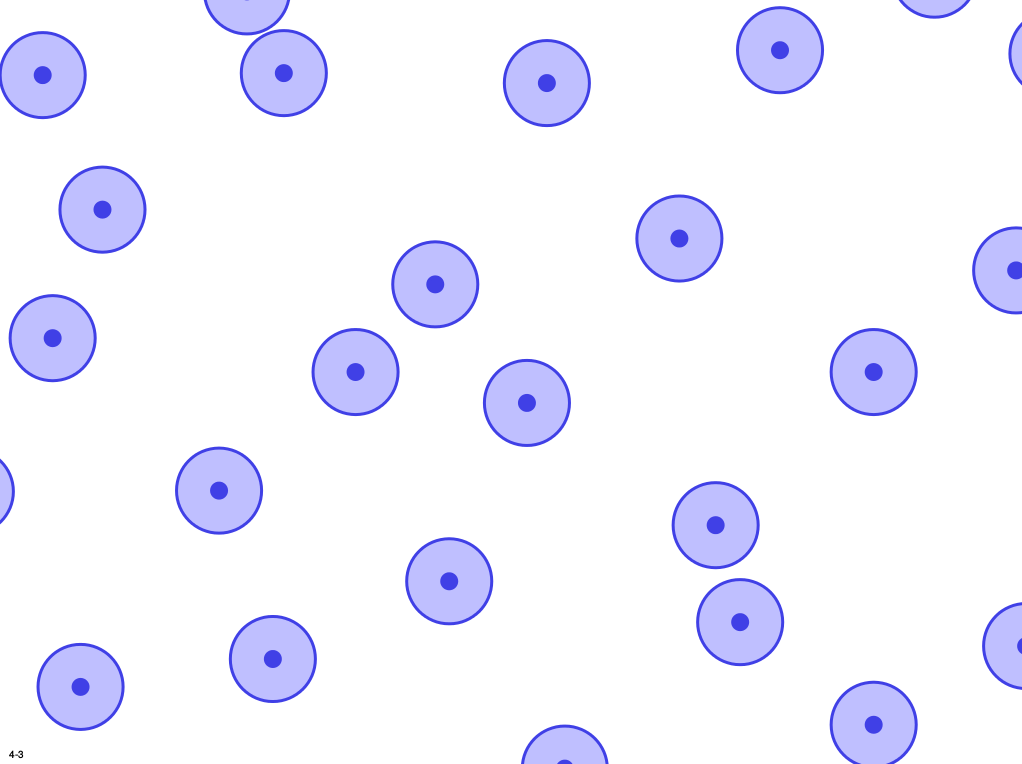
\includegraphics[width=1.1\textwidth ,angle=90]{img/problem_given.png}}
\only<2>{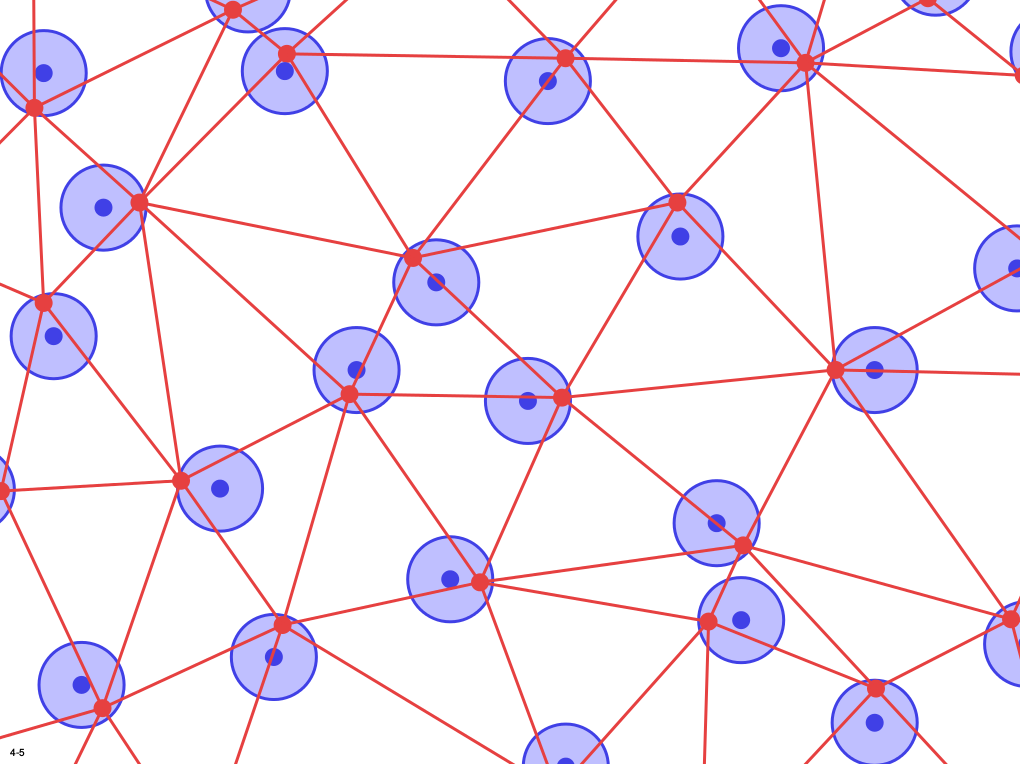
\includegraphics[width=1.1\textwidth ,angle=90]{img/problem_get.png}}
	\end{figure}


\end{columns}
\end{frame}

\begin{frame}
\frametitle{Outline}
\tableofcontents
\end{frame}

\section{Notions}
\frame{\tableofcontents[currentsection]}

\begin{frame}{Delaunay Triangulation}
\begin{figure}
		\centering
	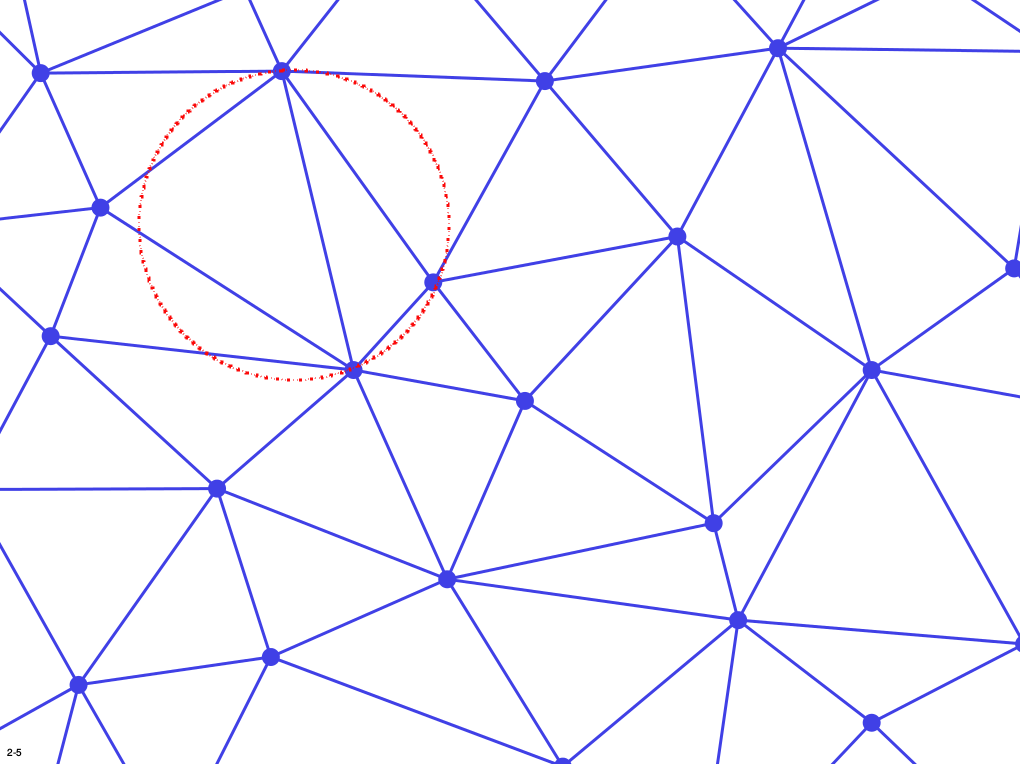
\includegraphics[scale=0.3]{img/delaunayTriangulation.png}
	\end{figure}
\end{frame}

\begin{frame}{Imprecise point}
\textbf{Imprecise point}: extending a point to some region
\begin{figure}
		\centering
	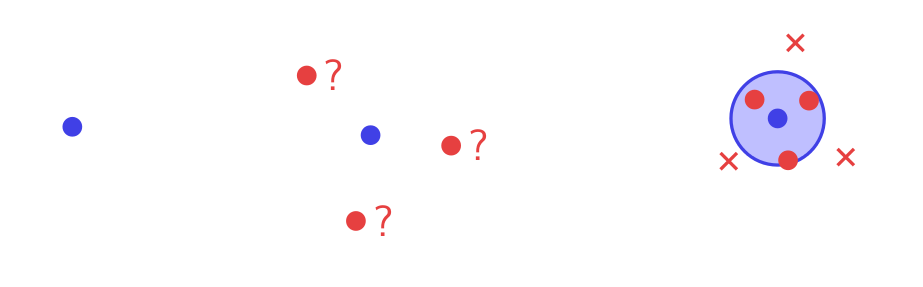
\includegraphics[width=\textwidth]{img/imprecise_point.png}
	\end{figure}
\pause
Supposing we have precise locations within the regions (point instances)
\end{frame}

\begin{frame}{Imprecise point}
\begin{itemize}
\item $|W| \rightarrow $ a set $W$
\item $|xy| \rightarrow $ distance between points x and y.
\item $DT_P \rightarrow $ Delaunay triangulation of set of points $P$
\item $NNP(v) \rightarrow $ nearest neighbour graph of $v \in P$ in $P \setminus \{v\}$
\item $d°G(v) \rightarrow $ degree of point $v$ in graph $G$
\item $\dot{p} \rightarrow $ the center of imprecise point $p$
\item $\hat{p} \rightarrow $ an instance of imprecise point p.
\item $S, \dot{S}, \hat{S} $ analogously being the sets of points 
\item $D(p) \rightarrow $ the disk with center $p$ and radius $||\dot{p} NN\dot{S}(\dot{p})|| + 1$, in case of disjoint unit disks $S$
\item $W(q) = \{p \in S \setminus {q}; \hat{q} \in D(p)\}$ 
\end{itemize}

\end{frame}


\section{Algorithm}
\frame{\tableofcontents[currentsubsection]}
\begin{frame}{Preprocessing}

\end{frame}

\begin{frame}{Instance processing}

\end{frame}


\section{Analysis}
\frame{\tableofcontents[currentsection]}

\begin{frame}

\end{frame}

\begin{frame}{Complexity -- unit disjoint regions}
Expected cost of building $D_{\hat{S}}$ is linear.
\\
\textit{Proof:} by Backward analysis, cost of adding last point $\hat{p}$:\\
3 steps:
\begin{itemize}
\item visit triangles incident to $\hat{x} \in DT_{\hat{S} \setminus \{\hat{p}\}}$
\item visit triangles crossed by line segment $\hat{x}\hat{p}$
\item update triangulation to $DT_{\hat{S}}$
\end{itemize}

Together: 
\begin{gather*}
d°_{DT_{\hat{S}}}(\hat{x}) + 3 \times d°_{DT_{\hat{S}}}(\hat{p}) + \sum_{\hat{q} \in D(p)} d°_{DT_{\hat{S}}}(\hat{q})
\end{gather*}

\end{frame}

\begin{frame}{Complexity -- unit disjoint regions}

\begin{itemize}
\item The expected degree of $\hat{p}$ in $DT_{\hat{S}}$ is less than or equal to 6
\item The expected degree of $\hat{x}$ in $DT_{\hat{S}}$ is less than or equal to 36
\item The expected value of $\sum_{\hat{q}\in D(P)} d°_{DT_{\hat{S}}}(\hat{q})$ is less than or equal to 132.
\begin{itemize}
\item proof using lemma 1
\end{itemize}
\end{itemize}

\textit{Therefore complexity of adding last point is constant.} $\blacksquare$
\end{frame}

\section{Experiment}
\frame{\tableofcontents[currentsection]}
\begin{frame}{Experiment}
\begin{itemize}
\item Imprecise points vs. classical Delaunay triangulation
\item Point sets: Random discs, Brownian motion, Random Balls, 3D noisy data
\item running time and \# triangles visited
\end{itemize}
\end{frame}

\begin{frame}{Running time}
\begin{tabular}{|l||l|l|l|l|l|l|}
\hline
2D random \\
imprecise points & \multicolumn{6}{|c|}{running time  ($\mu s$) per point}\\
 \hline \hline
    n & $10^3$ & $10^4$ & $10^5$ & $10^6$ & $10^7$ & $10^8$\\\hline
    spatial sort & $1.1$ & $0.85 $ & $0.83 $ & $0.90 $ & $1.0 $ & $1.13$\\\hline
    Delaunay hierarchy & $1.8$ & $1.6$ & $2.8 $ & $5.78 $ & $9.0$ & $13$\\\hline
    Skewchuch & $0.96 $ & $1.12$ & $1.05 $ & $1.61 $ & $2.4$ &\\\hline
    hint random order & $0.9 $ & $0.88 $ & $1.2 $ & $2.9 $ & $3.8$ & $5.4$\\\hline
    \textbf{hint spatial sort} & $1.0 $ & $0.79$ & $0.59$ & $0.61 $ & $0.61 $ & $0.62$\\\hline
\end{tabular}
\end{frame}

\begin{frame}{Running time}
\begin{tabular}{|l||l|l|l|l|l|l|}
\hline
2D Brownian \\
motion & \multicolumn{6}{|c|}{running time  ($\mu s$) per point}\\
 \hline \hline
    n & $10^3$ & $10^4$ & $10^5$ & $10^6$ & $10^7$ & $10^8$ \\\hline
    spatial sort & $0.78$ & $0.78 $ & $0.88 $ & $0.96 $ & $1.12 $ & $1.20$\\\hline
    \textbf{hint spatial sort} & $0.73 $ & $0.69$ & $0.79$ & $0.81 $ & $0.83 $ & $0.82$\\
    \hline
\end{tabular}
\end{frame}

\begin{frame}{Running time}
\begin{tabular}{|l||l|l|l|l|l|}
\hline
3D random \\
imprecise points & \multicolumn{5}{|c|}{running time  ($\mu s$) per point}\\
 \hline \hline
    n & $10^3$ & $10^4$ & $10^5$ & $10^6$ & $10^7$ \\\hline
    spatial sort & $9.0$ & $7.6 $ & $8.0$ & $8.2$ & $8.4$\\\hline
    Delaunay hierarchy & $11$ & $9.7$ & $18$ & $25$ & $33$\\\hline
    hint random order & $9.2 $ & $7.8 $ & $14.2 $ & $19 $ & $23$ \\\hline
    \textbf{hint spatial sort} & $9.5$ & $7.5$ & $7.8$ & $7.9$ & $8.0$\\\hline
\end{tabular}
\end{frame}

\begin{frame}{Running time}
\begin{tabular}{|l||l|l|l|l|}
\hline
3D noisy sample \\
of scanned models& \multicolumn{4}{|c|}{running time  ($\mu s$) per point}\\
 \hline \hline
    n & $10^3$ & $10^4$ & $10^5$ & full size ($2 \cdot 10^6$ points)\\\hline
    spatial sort & $7$ & $8.2$ & $8.6$ & $8.9$\\\hline
    \textbf{hint spatial sort} & $7$ & $7.5$ & $7.7$ & $7.5$\\\hline
\end{tabular}
\end{frame}

\begin{frame}{Visited triangles}
\begin{tabular}{|l||l|l|l|l|l|l|}
\hline
2D random \\
imprecise points & \multicolumn{6}{|c|}{number of visited triangles per point}\\
 \hline \hline
    n & $10^3$ & $10^4$ & $10^5$ & $10^6$ & $10^7$ & $10^8$\\\hline
    spatial sort & $3.74$ & $3.64 $ & $3.71 $ & $3.67 $ & $3.55 $ & $3.71$\\\hline
    Delaunay hierarchy & $24$ & $28$ & $29$ & $38$ & $45$ & $47$\\\hline
    hint random order & $2.83 $ & $2.8 $ & $2.77 $ & $2.75 $ & $2.75$ & $2.74$\\\hline
    \textbf{hint spatial sort} & $2.82$ & $2.80$ & $2.77$ & $2.76$ & $2.75$ & $2.75$\\\hline
\end{tabular}
\end{frame}

\begin{frame}{Visited triangles}
\begin{tabular}{|l||l|l|l|l|l|l|}
\hline
2D Brownian \\
motion & \multicolumn{6}{|c|}{number of visited triangles per time step}\\
 \hline \hline
    n & $10^3$ & $10^4$ & $10^5$ & $10^6$ & $10^7$ & $10^8$\\\hline
    spatial sort & $3.81$ & $3.68 $ & $3.77 $ & $3.72 $ & $3.62 $ & $3.78$\\\hline
    \textbf{hint spatial sort} & $2.77$ & $2.77$ & $2.77$ & $2.77$ & $2.77$ & $2.77$\\\hline
\end{tabular}
\end{frame}

\begin{frame}{Visited triangles}
\begin{tabular}{|l||l|l|l|l|l|}
\hline
3D random \\
imprecise points & \multicolumn{5}{|c|}{number of visited triangles per point}\\
 \hline \hline
    n & $10^3$ & $10^4$ & $10^5$ & $10^6$ & $10^7$ \\\hline
    hint random order & $5.2 $ & $5.3 $ & $5.3$ & $5.2$ & $5.2$\\\hline
    spatial sort & $6.3$ & $6.6$ & $6.6$ & $6.6$ & $6.6$ \\\hline
    Delaunay hierarchy & $21$ & $29$ & $34$ & $42$ & $50$\\\hline
    \textbf{hint spatial sort} & $4.4$ & $4.6$ & $4.5$ & $4.5$ & $4.4$\\\hline
\end{tabular}
\end{frame}

\begin{frame}{Visited triangles}
\begin{tabular}{|l||l|l|l|l|}
\hline
3D noisy sample \\
of scanned models& \multicolumn{4}{|c|}{number of visited triangles per point}\\
 \hline \hline
    n & $10^3$ & $10^4$ & $10^5$ & full size ($2 \cdot 10^6$ points)\\\hline
    spatial sort & $7.0$ & $8.0$ & $8.6$ & $9.5$\\\hline
    \textbf{hint spatial sort} & $5.7$ & $6.0$ & $6.1$ & $6.4$\\\hline
\end{tabular}
\end{frame}

\begin{frame}{Conclution}

\end{frame}

\begin{frame}
\centering
\huge{Do you have any questions?}\\
\pause
\vspace*{1.5cm}
\centerline{\large{Thank you for your attention.}}
\end{frame}

\begin{frame}{Bibliography}
\bibliographystyle{plain}  
\nocite{*}
\bibliography{bibliography}
\end{frame}
\end{document}